% Section content template for individual Educative lessons
% This file contains the actual content for a specific section
% Generated from Educative API section content

% Section: Use Case Diagram for the Meeting Scheduler
% Section ID: 6566425982664704
% Section Slug: use-case-diagram-for-the-meeting-scheduler
% Generated: 2025-12-12T13:05:55.067911

Let's build the use case diagram for the meeting scheduler and understand the relationships between its main actors and core functions. First , we'll define the key elements of our system, followed by the full set of use cases and their relationships.

\subsection{System}\label{sQvpPOxXVjYK9n1Pk7YHQ}
\\
Our system is the meeting scheduler, responsible for organizing meetings by managing rooms, times, invitations, participant responses, and calendar updates.

\subsection{Actors}\label{sIu0GUc5o_4jhcmRtOkWa}
\\
Now, we'll define the main actors of the meeting scheduler.

\subsubsection{Primary actors}\label{7JcZBu97wGrjDeEiFlgHy}

\begin{itemize}
\item
\protect\phantomsection\label{Tu4IQdKFjW4QDUxsBzI_r}
\textbf{Organizer:} Schedules new meetings, cancels existing ones, books and releases meeting rooms, and manages participant lists.
\item
\protect\phantomsection\label{6v8LtVIBCPk_jTHbzYCUF}
\textbf{Participant:} Receives meeting invitations, accepts or declines invites, and manages their calendar by attending or withdrawing from meetings.
\end{itemize}

\subsection{Use cases}\label{o5G9nJkAGwGof-Tx15M4Y}
\\
In this section, we'll define the use cases for the meeting scheduler. We have listed the use cases according to their interactions with a particular actor.

\subsubsection{Organizer}\label{D22J7NC9_wT__idxntpE6}

\begin{itemize}
\item
\protect\phantomsection\label{-VGQ2LkiJM8z4t-uJgDW1}
\textbf{Schedule meeting:} The organizer can create a new meeting by specifying the date, time interval, participants, agenda, and booking a suitable meeting room.
\item
\protect\phantomsection\label{vMkOTcPRtTKk0KasT8h7N}
\textbf{Cancel meeting:} This option allows the organizer to cancel a previously scheduled meeting, freeing the reserved meeting room and notifying all invited participants.
\item
\protect\phantomsection\label{YSoRVsS6bTmd39UKYpnIS}
\textbf{Add participant to meeting:} Lets the organizer add new participants to an already scheduled meeting, triggers invitation notifications and updating participant calendars.
\item
\protect\phantomsection\label{mslLhZXz8VRQXuiA3_09j}
\textbf{Remove participant from meeting: ~} Permits the organizer to remove participants from a scheduled meeting, ensure that the removed users receive notifications and their calendars are updated.
\end{itemize}

\subsubsection{Participant}\label{2iZXgFJcybn501SNioA-I}

\begin{itemize}
\item
\protect\phantomsection\label{ZtDdjfsnkrPGbkl1Sh_9k}
\textbf{Accept invitation:} A participant can accept a meeting invitation, which updates their calendar and changes their response status in the meeting record.
\item
\protect\phantomsection\label{9oMjuE2RS-Zncw_ZKUKH_}
\textbf{Reject invitation:} This option allows a participant to decline a meeting invitation, which removes the meeting from their calendar and updates their response status in the meeting record.
\item
\protect\phantomsection\label{D-MzDyI1Mg2rP46dQj5iC}
\textbf{Attend meeting:} Represents the participant's attendance at a scheduled meeting.
\item
\protect\phantomsection\label{ps7tWqI9c_fMvifNi306D}
\textbf{Withdraw from meeting:} This option allows a participant to withdraw from a meeting they had previously accepted, updating their calendar and notifying the organizer.
\end{itemize}

\subsubsection{Meeting scheduler}\label{_7pl-PeJDGf9z0puKAg0x}

\begin{itemize}
\item
\protect\phantomsection\label{eNlDOYigga-pNepPra0ys}
\textbf{Send invite notification:} Sends notifications to participants when invited to a new or updated meeting.
\item
\protect\phantomsection\label{714ufQNyq6-RKXZnmgrym}
\textbf{Send cancellation notification:} Sends notifications to all participants when a meeting is canceled.
\item
\protect\phantomsection\label{mka7iMTKzwjhv-vWgemDV}
\textbf{Update calendar:} Automatically updates users' calendars whenever a meeting is created, updated, canceled, or when participant statuses change.
\item
\protect\phantomsection\label{L3AZaJWsHbbrdgk5dC0HX}
\textbf{Remove meeting from calendar:} A meeting entry is removed from a participant's calendar when they decline or withdraw from a meeting or when the meeting is canceled.
\item
\protect\phantomsection\label{WHRAUbOeIAApxqZi-6v9V}
\textbf{Book room:} Reserves a meeting room for a scheduled meeting.
\item
\protect\phantomsection\label{_3ZhsKAU6Fxl6dYM8Ca7q}
\textbf{Check room availability:} Verify if a meeting room is available and suitable for the desired time and participant count.
\item
\protect\phantomsection\label{qY-jRZ82ksIx798HwZ16X}
\textbf{Release room:} Frees a reserved meeting room when a meeting is canceled.
\end{itemize}

\subsection{Relationships}\label{GxbHka8cDwCLgPxUy01h5}
\\
This section describes the relationships between and among actors and their use cases.

\subsubsection{Associations}\label{DkU7xBwuzAyOwGbxDO5w3}
\\
The table below shows the association relationship between actors and their use cases.

\begin{center}
{\def\LTcaptype{none} % do not increment counter
\begin{longtable}[]{@{}
>{\raggedright\arraybackslash} p{(\linewidth - 4\tabcolsep) * \real{0.3333}}
>{\raggedright\arraybackslash} p{(\linewidth - 4\tabcolsep) * \real{0.3333}}
>{\raggedright\arraybackslash} p{(\linewidth - 4\tabcolsep) * \real{0.3333}}@{}}
\toprule\noalign{}
\endhead
\bottomrule\noalign{}
\endlastfoot
\begin{minipage}[t]{\linewidth}\raggedright
\textbf{Organizer}
\end{minipage} & \begin{minipage}[t]{\linewidth}\raggedright
\textbf{Participant}
\end{minipage} & \begin{minipage}[t]{\linewidth}\raggedright
\textbf{Meeting Scheduler}
\end{minipage} \\
\begin{minipage}[t]{\linewidth}\raggedright
Schedule meeting
\end{minipage} & \begin{minipage}[t]{\linewidth}\raggedright
Accept invitation
\end{minipage} & \begin{minipage}[t]{\linewidth}\raggedright
Send invite notification
\end{minipage} \\
\begin{minipage}[t]{\linewidth}\raggedright
Cancel meeting
\end{minipage} & \begin{minipage}[t]{\linewidth}\raggedright
Reject invitation
\end{minipage} & \begin{minipage}[t]{\linewidth}\raggedright
Send cancelation notification
\end{minipage} \\
\begin{minipage}[t]{\linewidth}\raggedright
Add participant to meeting
\end{minipage} & \begin{minipage}[t]{\linewidth}\raggedright
Attend meeting
\end{minipage} & \begin{minipage}[t]{\linewidth}\raggedright
Update calendar
\end{minipage} \\
\begin{minipage}[t]{\linewidth}\raggedright
Remove participant from meeting
\end{minipage} & \begin{minipage}[t]{\linewidth}\raggedright
Withdraw from meeting
\end{minipage} & \begin{minipage}[t]{\linewidth}\raggedright
Remove meeting from calendar
\end{minipage} \\
\multirow{3}{=}{\begin{minipage}[t]{\linewidth}\raggedright
\end{minipage}} & \multirow{3}{=}{\begin{minipage}[t]{\linewidth}\raggedright
\end{minipage}} & \begin{minipage}[t]{\linewidth}\raggedright
Book room
\end{minipage} \\
& & \begin{minipage}[t]{\linewidth}\raggedright Check room availability
\end{minipage} \\
& & \begin{minipage}[t]{\linewidth}\raggedright Release room
\end{minipage} \\
\end{longtable}
}
\end{center}

\subsubsection{Include}\label{hiBmBcihUPVWriL8STfTe}
\\
When an organizer schedules a meeting, they must first reserve a room, select participants, and set the meeting details. The system then sends invitations and updates the calendars of all invited participants. These actions are best represented using ``include'' relationships in the use case diagram:

\begin{itemize}
\item
\protect\phantomsection\label{WdN1O3NaN3ovA7Aw86gop}
Schedule meeting includes:

\begin{itemize}
\item
\textbf{Check room availability:} The system checks whether a room is available before booking a room.
\item
\textbf{Book room:} After confirming room availability, the system books a room for a meeting.
\item
\protect\phantomsection\label{6gcoOtviSLYgaJTNxRcF3}
\textbf{Add participant to meeting:} The system adds participants to the meeting once the room is confirmed.
\item
\textbf{Send invite notification:} Invite notifications are sent to all participants after the meeting is scheduled.
\item
\textbf{Update calendar:} The meeting has been added to each participant's calendar to reserve the time slot.
\end{itemize}
\end{itemize}
\\
When an organizer cancels a meeting, the system ensures the meeting room is released, all participants are notified, and the meeting is removed from their calendars:

\begin{itemize}
\item
\protect\phantomsection\label{qLt5Bvhyld1xwjHVjAnPj}
Cancel meeting includes:

\begin{itemize}
\item
\textbf{Release room:} The reserved room is made available for others once the meeting is canceled.
\item
\textbf{Send cancellation notification:} All participants are notified of the meeting cancellation.
\item
\textbf{Remove meeting from calendar:} The meeting is removed from the calendars of all invited participants.
\end{itemize}
\end{itemize}
\\
When an organizer adds a new participant to a meeting, the system must invite the new participant and update their calendar:

\begin{itemize}
\item
\protect\phantomsection\label{6gcoOtviSLYgaJTNxRcF3}
Add participant to meeting includes:

\begin{itemize}
\item
\textbf{Send invite notification:} The newly added participant is notified about their invitation.
\item
\textbf{Update calendar:} The meeting has been added to the new participant's calendar.
\end{itemize}
\end{itemize}
\\
When an organizer removes a participant from a meeting, the system must update the participant:

\begin{itemize}
\item
\protect\phantomsection\label{RsByaV6noViyFbfCUfPX9}
Remove participant from meeting includes:

\begin{itemize}
\item
\textbf{Send cancellation notification:} The removed participant is notified that they are no longer part of the meeting.
\item
\textbf{Remove meeting from calendar:} The meeting is removed from the participant's calendar.
\end{itemize}
\end{itemize}
\\
When a participant accepts a meeting invitation, the meeting is added to their calendar:

\begin{itemize}
\item
\protect\phantomsection\label{EphPGrhqzfqfBuHXySMoW}
Accept invitation includes:

\begin{itemize}
\item
\textbf{Update calendar:} The meeting appears in the participant's calendar.
\end{itemize}
\end{itemize}
\\
When a participant rejects a meeting invitation, the meeting is removed from their calendar:

\begin{itemize}
\item
\protect\phantomsection\label{IspvLalm2B5_38lOCKXa1}
Reject invitation includes:

\begin{itemize}
\item
\textbf{Remove meeting from calendar:} The meeting is removed from the participant's calendar if it was previously there.
\end{itemize}
\end{itemize}

\subsection{Use case diagram}\label{9TTCXZGN7jxEAR4zgGQkW}
\\
Here's the use case diagram of the meeting scheduler:

\begin{figure}[htbp]
 \centering
 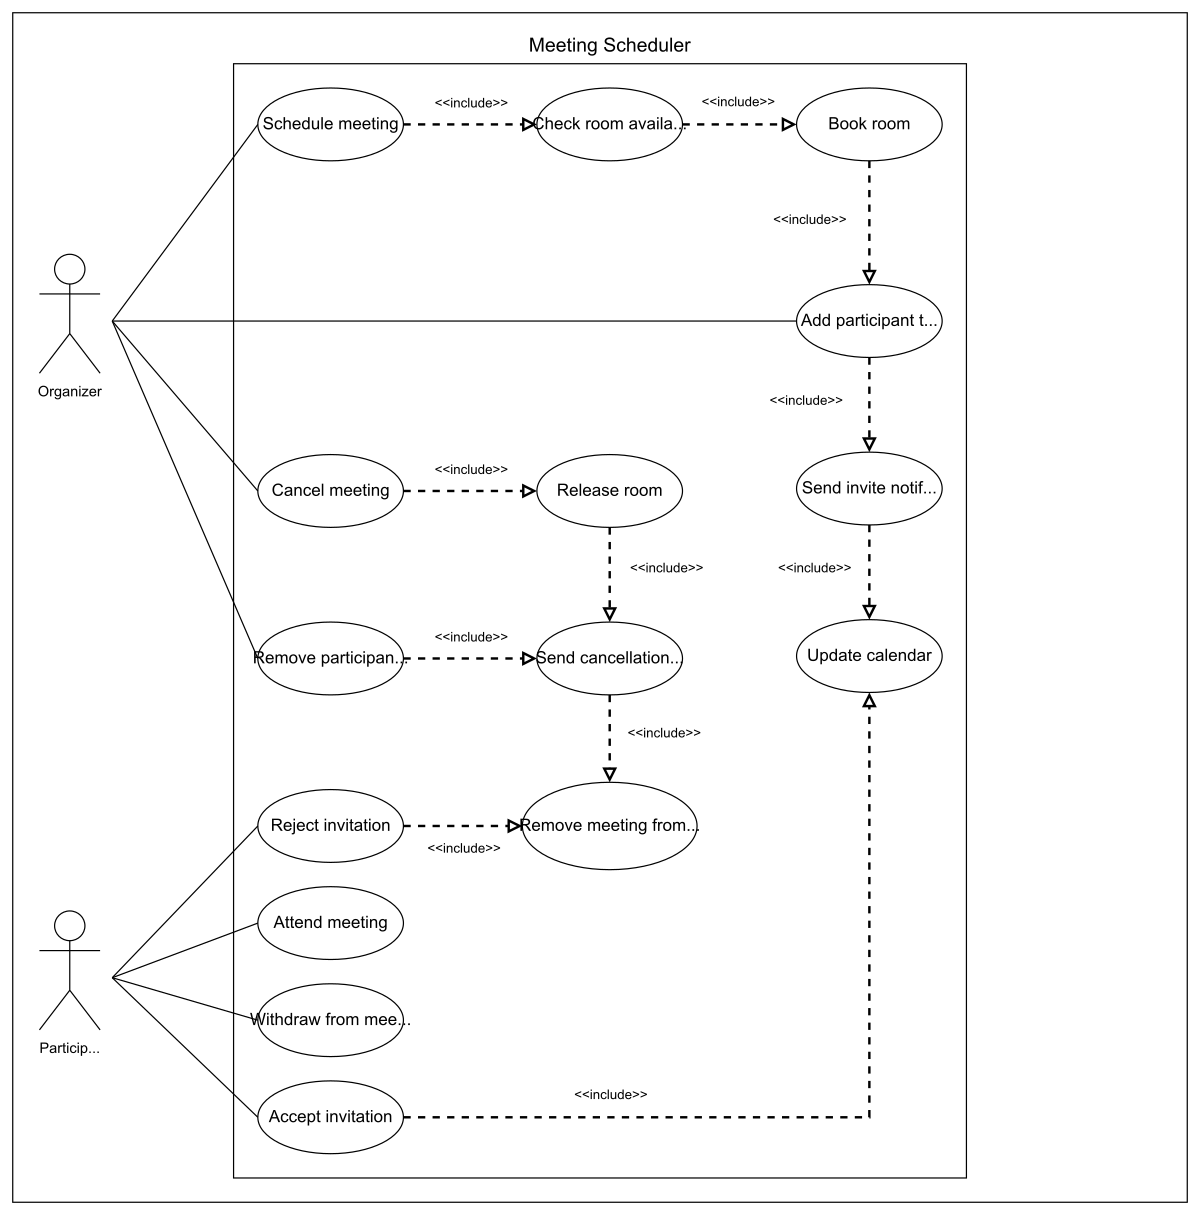
\includegraphics[width=0.5\textwidth]{Images/chapter_13/section_6566425982664704/4719484135669760.png}
 \caption{The use case diagram of the meeting scheduler}
\end{figure}

In the next lesson, we'll discuss the class diagram with a detailed explanation of all classes and their relationship with each other.

% End of section content